\chapter{Kravspecifikation}

\clearpage

% Indledning

\section{Indledning}
Gruppen vil udvikle et system til vanding af golfbaner. I forbindelse med stigende temperaturer bliver det mere kritisk, at vandingen af golfbaner sker på de rigtige tidspunkter, for at holde banen spilbar. For at spare på ressourcerne er det også kritisk, ikke at spilde store mængder vand, på vanding af områder som ikke trænger til det. 

Med et system af intelligente enheder der arbejder autonomt, men som modtager indstillinger for vandingen fra en Master, styres vandingen på hele Golfbanen centralt. På denne måde sparer man arbejdstid for greenkeeperen og vandingen sker kun når det er nødvendigt. Systemet kaldes for EasyWater8000. 
Normalt vil man placere en af disse enheder ved hvert hul på golfbanen og lave et netværk af sensorer lokalt til denne enhed. Enheden kan herved overvåge området og vande hvis nødvendigt. Alle enhederne forbindes til et netværk, som er koblet sammen med en masterenhed. Grænseværdierne, for f.eks. jordfugtigheden, der afgør hvornår enheden, skal påbegynde vanding kommer fra Master og styres igennem denne af greenkeeperen. 


\begin{figure}[ht] \centering
\fbox{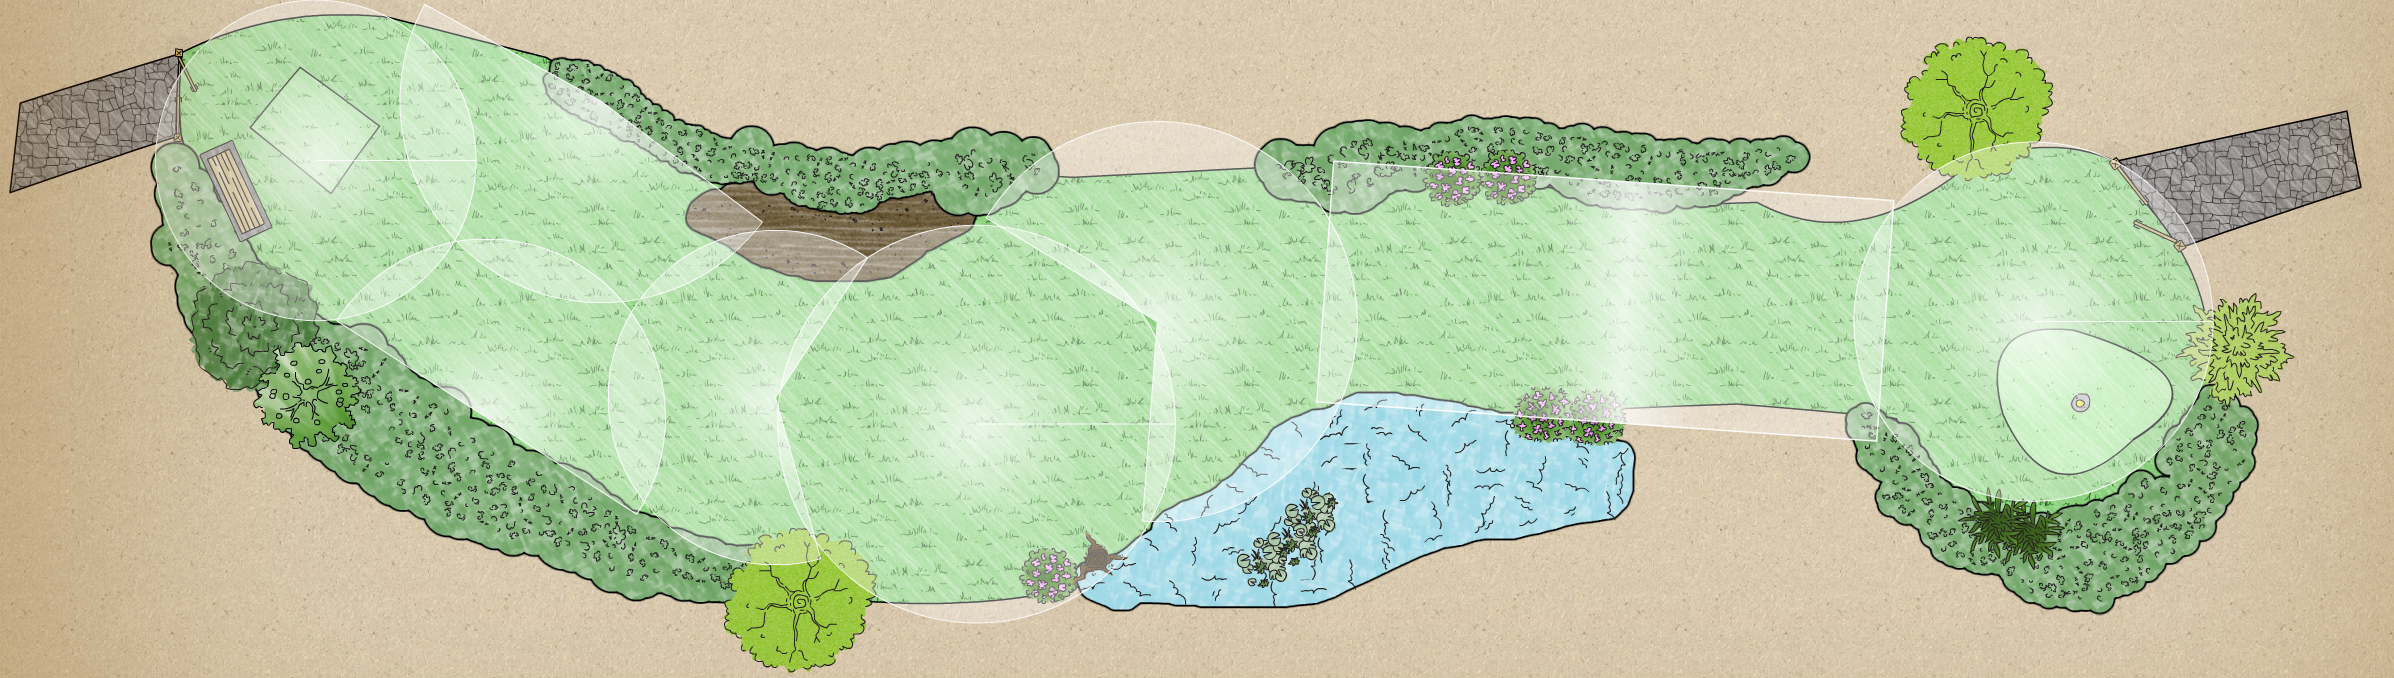
\includegraphics[height=4.1cm]{filer/indledning/billeder/hul_med_sprinkler}}
\caption{Overblik af golfhul med system}
\label{fig:systemoverblik}
\end{figure}

Figur \ref{fig:systemoverblik} illustrerer et hul på en given golfbane. Dette hul er inddelt i 11 områder, med hver sin sprinkler. Spinklere er markeret ved halv til helcirkler på figuren. Til venstre på figuren ses tee-stedet med tilhørende indgang. Ved denne indgang er der placeret en bevægelsessensor, som sørger for at der ikke kan vandes på banen, når der er spillere. 

Oversigt over blokkene i systemet kan ses i figur \ref{fig:bloksystemoverblik}. De tre hovedbegreber for systemet er Master, som er hovedenheden baseret på Devkit8000. Enhed som er de autonome undersystemer på hvert hul, hvor hovedenheden er PSoC, og Komponentpakker som er et begreb for pakken med temperatur- og fugtsensor samt sprinkler. Disse er distribueret ud på selve golfhullet.

\begin{figure}[ht] \centering
\fbox{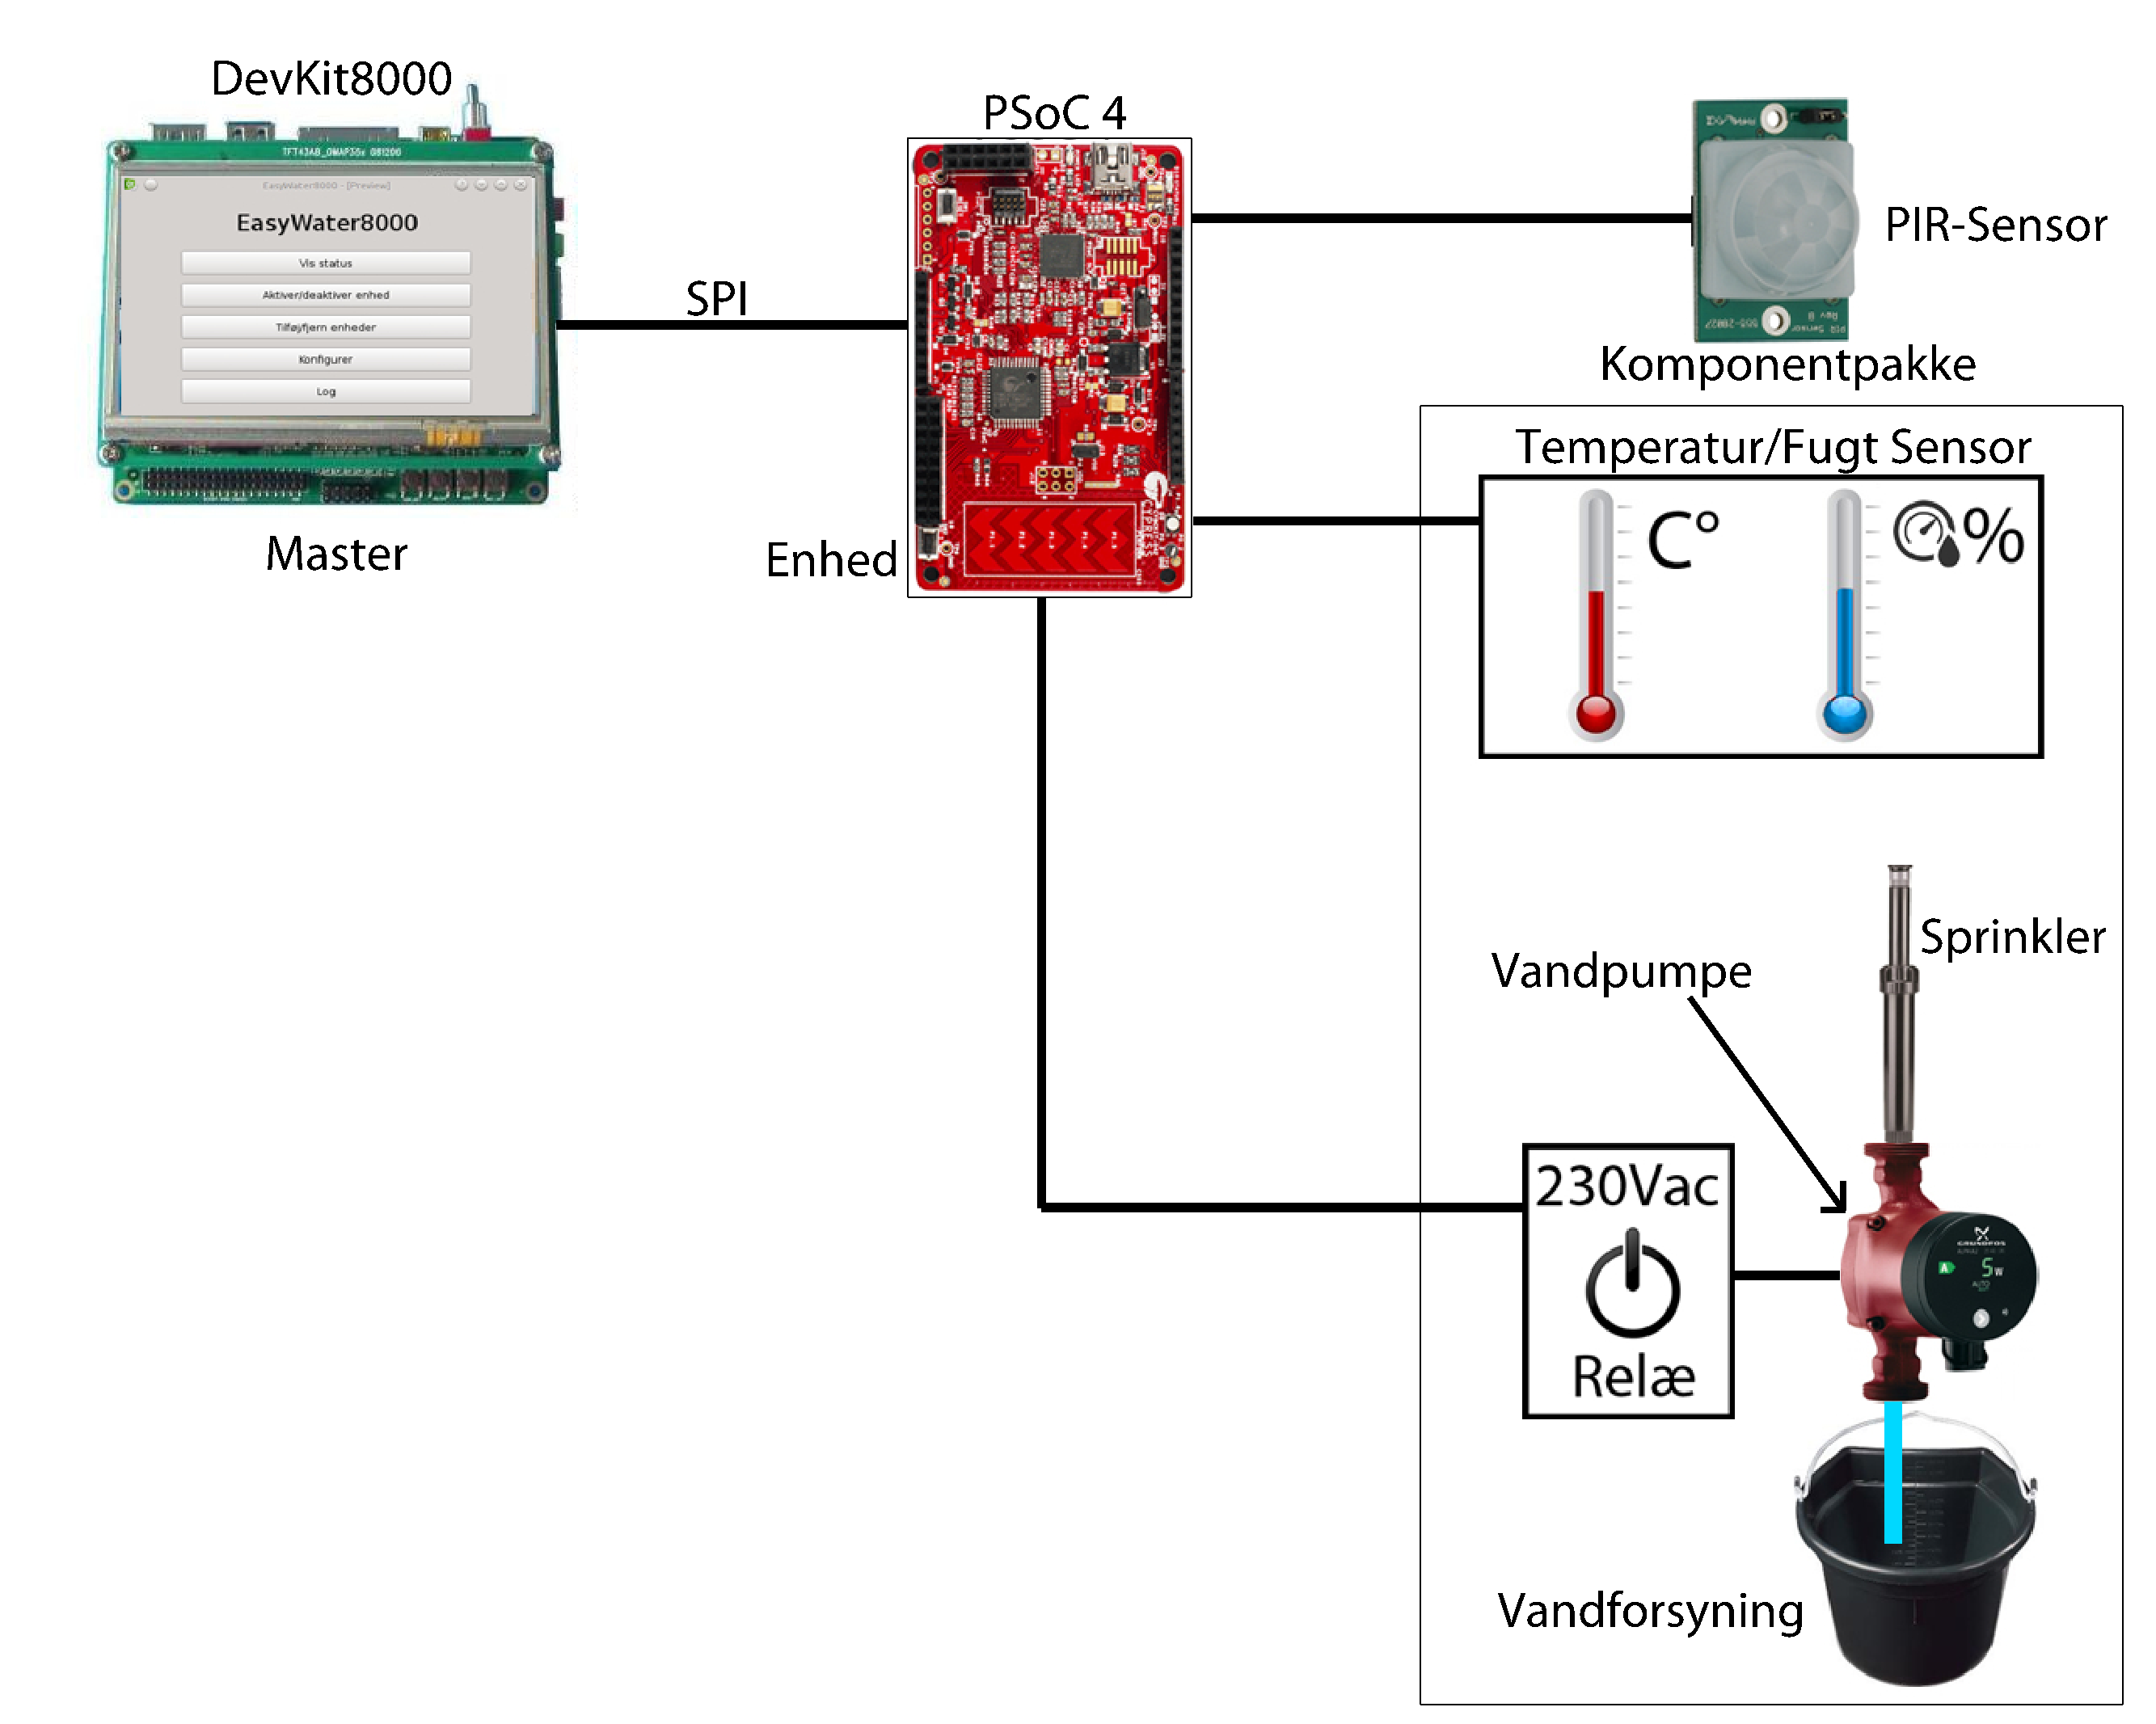
\includegraphics[height=10cm]{filer/indledning/billeder/vandingssystem}}
\caption{Systemoverblik}
\label{fig:bloksystemoverblik}
\end{figure}

En Enhed består altså af:
\begin{enumerate}
\item Fugtighedssensor(er)
\item Temperatursensor(er)
\item Bevægelsessensor(er) 
\item Sprinkler(e)
\item PSoC controller board
\end{enumerate}

Fugt- og temperatursensorerne registrerer banens behov for vanding. Bevægelsessensoren registrerer om der er spillere på det pågældende hul. Sprinkleren sørger for vandingen når der skal vandes. Denne skjules nede i græsset og kommer op når vandingen skal være aktiv.
PSoC4 controller-boardet bliver hjernen i Enheden. Denne holder styr på de generelle funktioner for Enheden så som udlæsning af data, aktivering af sprinkler m.v.

% Aktører

\section{Aktører}
Her beskrives systemets aktører. Disse vil blive refereret til, i de efterfølgende usecase-beskrivelser.


%% !!! Aktør kontekst diagram !!!
\begin{figure}[htbp] \centering
\fbox{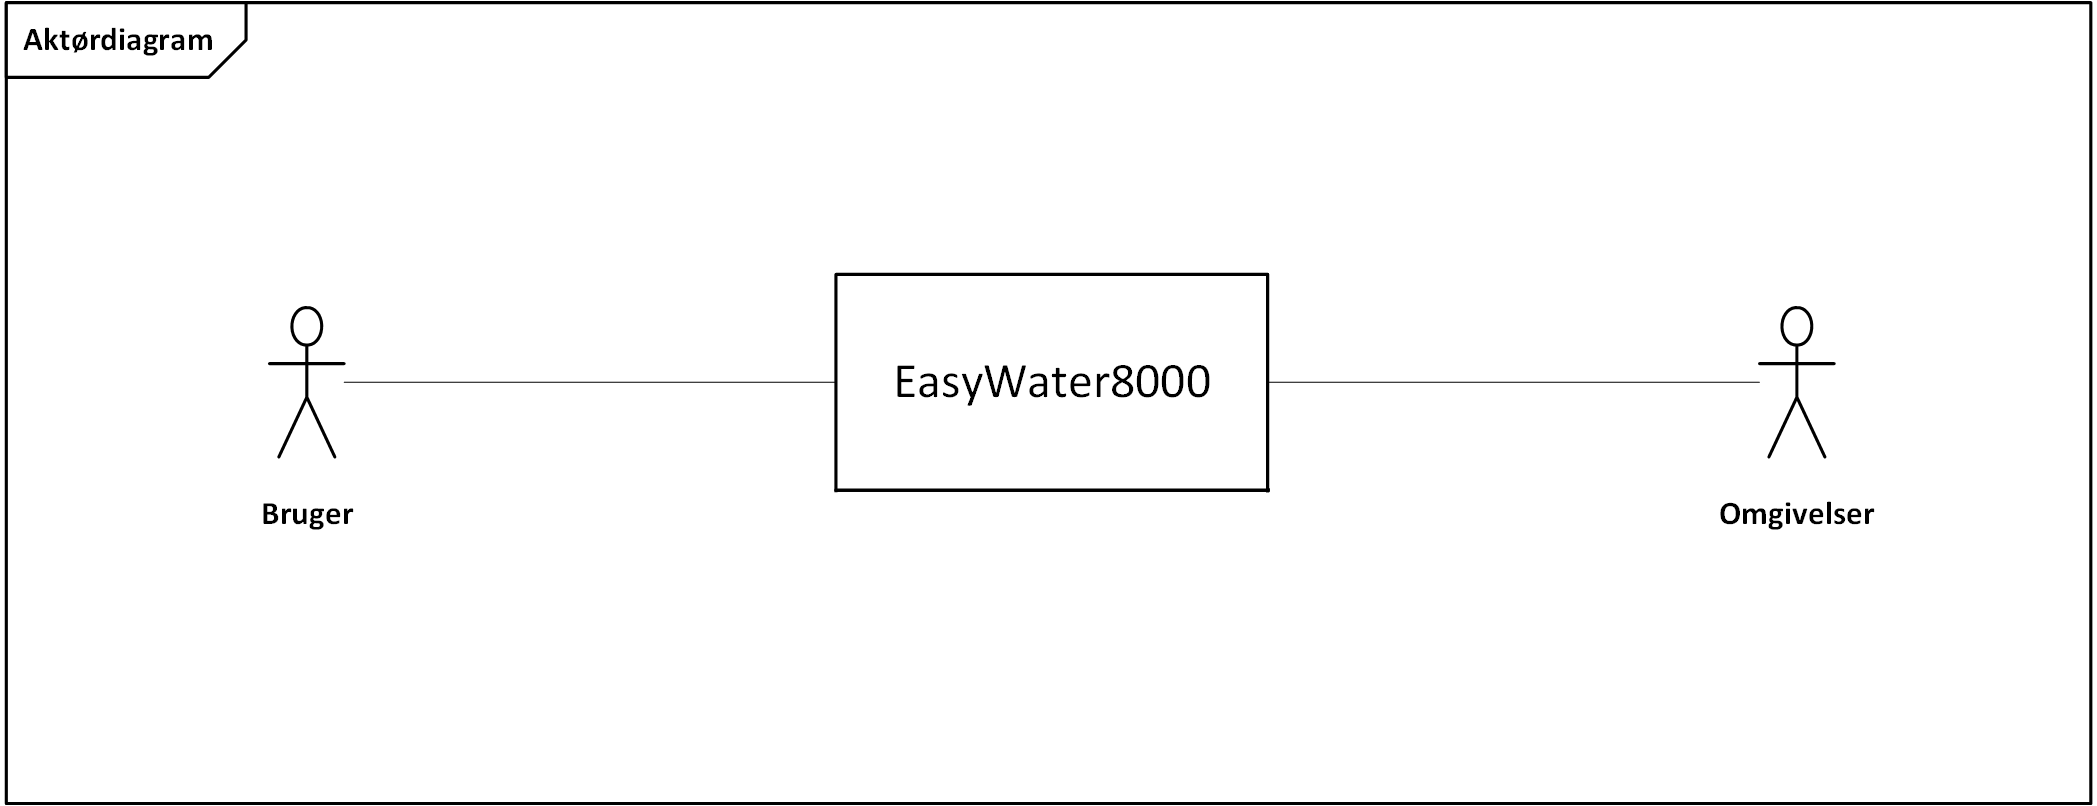
\includegraphics[width=0.9\textwidth]{filer/kravspec/visio/Kontekst_Diagram}}
\caption{Kontekst diagram}
\label{lab:kontekstdiagram}
\end{figure}

\begin{table}[!htbp] \centering
	\begin{tabular}{|p{2.5cm}|p{11.5cm}|}
	\hline
		\textbf{Aktør navn} & \textbf{Beskrivelse} \\\hline
		Bruger & Bruger-aktøren vil normalt være greenkeeperen. Det er vedkommende som kontrollerer og betjener systemet. (Primær) \\\hline

		Golfbane & De almene omgivelser på golfbanen, som har indflydelse på systemets sensorer. Det indebærer temperatur, fugtighed og bevægelser i områderne omkring systemet. (Sekundær) \\\hline
	\end{tabular}
\end{table}



% Usecases

\section{Usecases}

Her følger en dybere beskrivelse af systemets opbygning og måde at virke på. Dette gøres med fulde usecase beskrivelser hvor systemets virkning er beskrevet i detaljer.

\begin{figure}[!htbp] \centering
\vspace*{\fill}
\includegraphics[width=\textwidth]{filer/kravspec/visio/Usecase_Diagram}
\caption{Usecase diagram}
\label{lab:usecasediagram}
\vspace*{\fill}
\end{figure}

%% !!! Use case diagram !!!
%
%\begin{figure}[!htbp] \centering
%\section{Usecases}
%\vspace*{\fill}
%\includegraphics[width=\textwidth]{billeder/diagrammer/Usecase_Diagram}
%\caption{Usecase diagram}
%\label{lab:usecasediagram}
%\vspace*{\fill}
%\end{figure}

% UC1: Tilføj/fjern enhed

\subsection{UC1: Tilføj/fjern enhed}
\begin{center} \centering \label{UC1}
	\begin{longtable}{|p{5cm}|p{9cm}|}  %% Longtable = forsætter på næste side
	\hline
		\multicolumn{2}{|l|}{\textbf{UC1: Tilføj\slash fjern enhed}} \\\hline %% HUSK UCECASE NUMMER + NAVN
		\endfirsthead
		
		\multicolumn{2}{l}{...fortsat fra forrige side} \\ \hline %% Til LONGTABLE
		\multicolumn{2}{|l|}{\textbf{UC1: Tilføj\slash fjern enhed}} \\\hline %% HUSK UCECASE NUMMER + NAVN
		\endhead	
		
		\textbf{Mål}								&Bruger kan tilføje eller fjerne Enheder fra systemet			\\\hline
		\textbf{Initialisering}					&Bruger														\\\hline
		\textbf{Aktører og Stakeholders}			&Bruger(Primær)												\\\hline 
		\textbf{Referencer}						&Ingen														\\\hline
		\textbf{AASH}							&1															\\\hline
		\textbf{Efterfølgende tilstand}			&Ønsket Enhed er tilføjet eller fjernet fra systemet		\\\hline
		\textbf{Hovedforløb}					
			&\begin{enumerate}
	
				\item Bruger vælger ''Tilføj eller fjern enhed'' i hovedmenuen
				
				\item En liste af opsatte enheder præsenteres på skærmen				
				
				\item \label{uc1valg} Bruger vælger ''Tilføj''
				
				\begin{enumerate}
					\item \label{uc1indtast} Master beder bruger om at indtaste informationer
					
					\item \label{uc1indtast_fejl} Bruger indtaster hul-nr., adresse og parametre på Enhed
										
					\item Enhed forbindes til kommunikationsnetværket
					
					\item \label{uc1verif} Master verificerer forbindelsen til Enhed
						
					\textbf{[Undtagelse \ref{uc1verif}.a]} \newline
					Enheden kan ikke verificeres
					
					\item Master tilføjer Enhed til systemet

				\end{enumerate}

				\item Bruger vælger celle og trykker ''Fjern''

				\begin{enumerate}

					\item Master deaktiverer Enhed
					
					\item Master sletter Enhed fra systemet
				
				\end{enumerate}
				
				\item Master opdaterer liste med opsatte enheder
				
				\item Bruger kan returnere til hovedmenuen eller opsætte ny enhed (Gå til UC1.\ref{uc1valg})
			\end{enumerate}\\\hline
		\textbf{Undtagelser}
			&\begin{enumerate}[label=\ref{uc1verif}.a]
				
				\item Master viser fejlbesked angående verificering af enheden. Bruger kan forsøge igen (Gå til UC1.\ref{uc1verif} eller vælge ''Tilbage'')

			\end{enumerate}														\\\hline
	\end{longtable} 
\end{center}

%% TIPS:
%% LABEL TIL PUNKT: \label{labelnavn}
%% REFERENCE: \ref{labelnavn}

% UC2: Config

\subsection{UC2: Config}
\begin{center} \centering
	\begin{longtable}{|p{6cm}|p{8cm}|}  %% Longtable = forsætter på næste side
	\hline
		\multicolumn{2}{|l|}{\textbf{UC2: Aktiver/deaktiver}} \\\hline %% HUSK UCECASE NUMMER + NAVN
		\endfirsthead
		
		\multicolumn{2}{l}{...fortsat fra forrige side} \\ \hline %% Til LONGTABLE
		\multicolumn{2}{|l|}{\textbf{UC2: Aktiver/deaktiver}} \\\hline %% HUSK UCECASE NUMMER + NAVN
		\endhead	
		
		\textbf{Mål}								&At bruger kan aktivere og/eller deaktivere enheder			\\\hline
		\textbf{Initialisering}					&Bruger			\\\hline
		\textbf{Aktører og Stakeholders}			&Bruger(primær), PsoC(sekundær), devkit8000(sekundær)			\\\hline
		\textbf{Referencer}						&Ingen			\\\hline
		\textbf{Antal af samtidige hændelser}	&1			\\\hline
		\textbf{Forudsætning}					&devkit8000 er opsat og systemet er idel. Seriel bus er intakt.			\\\hline
		\textbf{Efterfølgende tilstand}			&Ingen			\\\hline
		\textbf{Hovedforløb}					
			&\begin{enumerate}
	
				\item Bruger logger ind på devkit8000
				
				\item Bruger vælger aktiver/deaktiver i hovedmenuen
				
				\item Bruger vælger aktiver eller deaktiver efter ønske
				
				\item Bruger indtaste adresse på valgte enhed for at aktivere eller deaktivere denne
	
			\end{enumerate}\\\hline
	\end{longtable}
	\label{UC2} 
\end{center}

%% TIPS:
%% LABEL TIL PUNKT: \label{labelnavn}
%% REFERENCE: \ref{labelnavn}

% UC3: Aktiver/deaktiver

\subsection{UC3: Aktiver/deaktiver}
\begin{center} \centering \label{UC3} 
	\begin{longtable}{|p{5cm}|p{9cm}|}  %% Longtable = forsætter på næste side
	\hline
		\multicolumn{2}{|l|}{\textbf{UC3: Aktiver/deaktiver}} \\\hline %% HUSK USECASENUMMER + NAVN
		\endfirsthead
		
		\multicolumn{2}{l}{...fortsat fra forrige side} \\ \hline %% Til LONGTABLE
		\multicolumn{2}{|l|}{\textbf{UC3: Aktiver/deaktiver}} \\\hline %% HUSK USECASENUMMER + NAVN
		\endhead	
		
		\textbf{Mål}								&At aktivere / deaktivere Enhed	\\\hline
		\textbf{Initialisering}					&Bruger				\\\hline
		\textbf{Aktører og Stakeholders}			&Bruger(Primær)		\\\hline
		\textbf{Referencer}						&Ingen				\\\hline
		\textbf{AASH}							&1					\\\hline
		\textbf{Forudsætning}					&Master er opsat og systemet kører \newline
												 Forbindelsen er intakt	\\\hline
		\textbf{Efterfølgende tilstand}			&Enhedstilstand ændres aktiv/deaktiv\\\hline
		\textbf{Hovedforløb}					
			&\begin{enumerate}
	
	
				\item Bruger vælger ''aktiver/deaktiver'' i hovedmenu
				
				\item Bruger markerer enhed ud fra liste af opsatte enheder
				
				\item \label{uc3aktiver} Bruger vælger ''Aktiver'' eller ''Deaktiver'' for at ændre enheden\newline
				\textbf{[Undtagelse \ref{uc3aktiver}.a]} Bruger vælger ''Afbryd''
				
				\item Master udskriver på dennes skærm, at ønsket Enhed er aktiveret eller deaktiveret		
			
				\item Bruger vælger ''Afslut''
				
				\item Master viser hovedmenu	
	
			\end{enumerate}\\\hline
			
		\textbf{Undtagelser}
			&\begin{enumerate}[label=\ref{uc3aktiver}.a]
				
				\item Bruger vælger ''Afbryd''
				
					\subitem Master viser hovedmenu
			\end{enumerate}\\\hline			
			
	\end{longtable}
\end{center}

%% TIPS:
%% LABEL TIL PUNKT: \label{labelnavn}
%% REFERENCE: \ref{labelnavn}

% UC4: Indsamle data

\subsection{UC4: Indsamle data}
\begin{center} \centering \label{UC4}
	\begin{longtable}{|p{5cm}|p{9cm}|}  %% Longtable = forsætter på næste side
	\hline
		\multicolumn{2}{|l|}{\textbf{UC4: Indsamle data}} \\\hline %% HUSK USECASENUMMER + NAVN
		\endfirsthead
		
		\multicolumn{2}{l}{...fortsat fra forrige side} \\ \hline %% Til LONGTABLE
		\multicolumn{2}{|l|}{\textbf{UC4: Indsamle data}} \\\hline %% HUSK USECASENUMMER + NAVN
		\endhead	
		
		\textbf{Mål}								&Indsamle data fra omkringliggende jord. Temperatur, fugt og bevægelse			\\\hline
		\textbf{Initialisering}					&Enhedstimer			\\\hline
		\textbf{Aktører og Stakeholders}			&Omgivelser				\\\hline
		\textbf{Referencer}						&UC8: Vanding		\\\hline
		\textbf{AASH}							&1 per Enhed			\\\hline
		\textbf{Forudsætning}					&Aktiv Enhed			\\\hline
		\textbf{Efterfølgende tilstand}			&Data gemt i Enhed 	\\\hline
		\textbf{Hovedforløb}					
			&\begin{enumerate}
	
				\item Sensorer måler kontinuert temperatur og fugt i banen og bevægelse på banen
				
				\item Enhed henter temperatur- og fugtdata samt vandingsstatus ved hver udløb af Enhedstimer
				
				\item Enhed gemmer data				
				
				\item Enhed modtager data ved bevægelse  
				
			\end{enumerate}\\\hline
	\end{longtable}
\end{center}

%% TIPS:
%% LABEL TIL PUNKT: \label{labelnavn}
%% REFERENCE: \ref{labelnavn}

% UC5: Vanding

\subsection{UC5: Vanding}
\begin{center} \centering \label{UC5} 
	\begin{longtable}{|p{5cm}|p{9cm}|}  %% Longtable = forsætter på næste side
	\hline
		\multicolumn{2}{|l|}{\textbf{UC5: Vanding}} 		\\\hline %% HUSK UCECASE NUMMER + NAVN
		\endfirsthead
		
		\multicolumn{2}{l}{...fortsat fra forrige side} 	\\ \hline %% Til LONGTABLE
		\multicolumn{2}{|l|}{\textbf{UC5: Vanding}} 		\\\hline %% HUSK UCECASE NUMMER + NAVN
		\endhead	
		
		\textbf{Mål}								&At vande trængende områder	\\\hline
		\textbf{Initialisering}					&Ingen						\\\hline
		\textbf{Aktører og Stakeholders}			&Golfbane(Primær)			\\\hline
		\textbf{Referencer}						&UC4: Indsamle data 			\\\hline
		\textbf{AASH}							&1							\\\hline
		\textbf{Forudsætning}					&Aktiv Enhed					\\\hline
		\textbf{Efterfølgende tilstand}			&Aktiv						\\\hline
		\textbf{Hovedforløb}					
			&\begin{enumerate}
				
				\item Enhed læser fugt- og temperaturværdier fra UC4: Indsamle data
				
				\item \label{uc5sprinkler} Vanding startes på områder med for lave værdier
				
					\textbf{[Undtagelse \ref{uc5sprinkler}a]} Bevægelse registreret
	
			\end{enumerate}\\\hline

		\textbf{Undtagelser}
			&\begin{enumerate}[label=\ref{uc5sprinkler}a.]
			
				\item Sprinkler deaktiveres i 30 minutter og herefter gentages hovedforløb	
			
			\end{enumerate}\\\hline
	\end{longtable}
\end{center}

%% TIPS:
%% LABEL TIL PUNKT: \label{labelnavn}
%% REFERENCE: \ref{labelnavn}

% UC6: Send log

\subsection{UC6: Send log}
\begin{center} \centering
	\begin{longtable}{|p{6cm}|p{8cm}|}  %% Longtable = forsætter på næste side
	\hline
		\multicolumn{2}{|l|}{\textbf{UC1: USECASENAVN}} \\\hline %% HUSK UCECASE NUMMER + NAVN
		\endfirsthead
		
		\multicolumn{2}{l}{...fortsat fra forrige side} \\ \hline %% Til LONGTABLE
		\multicolumn{2}{|l|}{\textbf{UC1: USECASENAVN}} \\\hline %% HUSK UCECASE NUMMER + NAVN
		\endhead	
		
		\textbf{Mål}								&Skriv her			\\\hline
		\textbf{Initialisering}					&Skriv her			\\\hline
		\textbf{Aktører og Stakeholders}			&Skriv her			\\\hline
		\textbf{Referencer}						&Skriv her			\\\hline
		\textbf{Antal af samtidige hændelser}	&Skriv her			\\\hline
		\textbf{Forudsætning}					&Skriv her			\\\hline
		\textbf{Efterfølgende tilstand}			&Skriv her			\\\hline
		\textbf{Hovedforløb}					
			&\begin{enumerate}
	
				\item %%Punkt 1
				
				\item %%Punkt 2
				
				\item %%Etc.
	
			\end{enumerate}\\\hline
	\end{longtable}
	\label{UC6} 
\end{center}

%% TIPS:
%% LABEL TIL PUNKT: \label{labelnavn}
%% REFERENCE: \ref{labelnavn}

% UC7: Tjek status

\subsection{UC7: Tjek status}
\begin{center} \centering \label{UC7}
	\begin{longtable}{|p{5cm}|p{9cm}|}  %% Longtable = forsætter på næste side
	\hline
		\multicolumn{2}{|l|}{\textbf{UC7: Udskriv log}} \\\hline %% HUSK USECASENUMMER + NAVN
		\endfirsthead
		
		\multicolumn{2}{l}{...fortsat fra forrige side} \\ \hline %% Til LONGTABLE
		\multicolumn{2}{|l|}{\textbf{UC7: Udskriv log}} \\\hline %% HUSK USECASENUMMER + NAVN
		\endhead	
		
		\textbf{Mål}								&Log udskrives på Masters skærm	\\\hline
		\textbf{Initialisering}					&Bruger 					\\\hline
		\textbf{Aktører og Stakeholders}			&Bruger(Primær)			\\\hline
		\textbf{Referencer}						&Ingen					\\\hline
		\textbf{AASH}							&1						\\\hline
		\textbf{Forudsætning}					&Aktiv Master		\\\hline
		\textbf{Efterfølgende tilstand}			&Hovedmenuen vises på Master	\\\hline
		\textbf{Hovedforløb}					
			&\begin{enumerate}
	
				\item Bruger vælger ''Udskriv log'' i hovedmenuen 
				
				\item Log udskrives på Masters skærm
				
				\item Bruger vælger ''Tilbage''
	
			\end{enumerate}\\\hline
	\end{longtable} 
\end{center}

%% TIPS:
%% LABEL TIL PUNKT: \label{labelnavn}
%% REFERENCE: \ref{labelnavn}

% UC8: Udskriv log

\subsection{UC8: Udskriv log}
\begin{center} \centering
	\begin{longtable}{|p{6cm}|p{8cm}|}  %% Longtable = forsætter på næste side
	\hline
		\multicolumn{2}{|l|}{\textbf{UC8: Vanding}} 		\\\hline %% HUSK UCECASE NUMMER + NAVN
		\endfirsthead
		
		\multicolumn{2}{l}{...fortsat fra forrige side} 	\\ \hline %% Til LONGTABLE
		\multicolumn{2}{|l|}{\textbf{UC8: Vanding}} 		\\\hline %% HUSK UCECASE NUMMER + NAVN
		\endhead	
		
		\textbf{Mål}								&At vande trængende områder	\\\hline
		\textbf{Initialisering}					&Bruger						\\\hline
		\textbf{Aktører og Stakeholders}			&Omgivelser(Primær)			\newline
												 Bruger(Sekundær)			\\\hline
		\textbf{Referencer}						&UC2: Aktivere/deaktivere 	\newline 
												 UC3: Planlagt vanding		\\\hline
		\textbf{Antal af samtidige hændelser}	&2							\\\hline
		\textbf{Forudsætning}					&Systemet kører				\\\hline
		\textbf{Efterfølgende tilstand}			&Trængende områder vandet	\\\hline
		\textbf{Hovedforløb}					
			&\begin{enumerate}
	
				\item Bruger aktivere (\ref{UC2}) automatisk vanding igennem Master
				
				\item Enhed læser fugt- og temperaturværdier
				
				\item \label{uc8sprinkler} Sprinkling startes på områder med for lave værdier
				
					\textbf{[Undtagelse \ref{uc8sprinkler}a]} Bevægelse registreret
				
				\item Master giver besked om planlagt vanding (\ref{UC3})
				
				\begin{enumerate}
					
					\item Alle sensorer ignoreres
					
					\item Alle områder vandes					
					
				\end{enumerate}
	
			\end{enumerate}\\\hline

		\textbf{Undtagelser}
			&\begin{enumerate}[label=\ref{uc8sprinkler}a.]
			
				\item Sprinkler deaktiveres i 5 minutter		
			
			\end{enumerate}\\\hline
	\end{longtable}
	\label{UC8} 
\end{center}

%% TIPS:
%% LABEL TIL PUNKT: \label{labelnavn}
%% REFERENCE: \ref{labelnavn}

%% Ikke-funktionelle krav

\section{Ikke-funktionelle krav}
% Ikke-funktionelle krav
\begin{enumerate}

\subsubsection*{Brugbarhed}
\item Opsætningen skal ske af autoriseret personale
\item UI skal kunne benyttes af bruger efter gennemlæst manual


\subsubsection*{Pålidelighed}
\item Levetid: 2 år uden hardware nedbrud
\item Software IDLE tid: minimum 1 måned uden restart


\subsubsection*{Ydeevne}
\item Master skal kunne håndtere minimum 18 enheder
\item Sprinkler skal kunne vande et areal afdækket af 360 grader med radius min. 3.5 m 
\item Der skal kunne tilføjes yderligere enheder efter opsætning af systemet


\subsubsection*{Vedligeholdelse}
\item Enheder skal være udskiftelige uden at det er nødvendigt at tilgå sensorer eller sprinkler
\item Sprinklere skal være let tilgængelige for personale


\subsubsection*{Generelle krav}
\item Al kommunikation sker via en seriel bus 


\subsubsection*{Enheder}
\item Enhed skal kunne operere autonomt efter denne er sat op fra Master
\item Enheder skal sende log information til Master efter hver udførte måling
\item Enheder skal sende log information til Master efter hver udført vanding

\end{enumerate}

\subsubsection*{Begrænsninger}
\begin{itemize}
\item Der udarbejdes en skaleret udgave, da vi ikke har adgang til en hel golfbane
\item Grundet tidsbegrænsninger udvikles der ikke et fuldt system 
\item Som minimum skal der produceres funktionel Master og én komplet Enhed
\item Systemet udvikles således, at der til hver sprinkler tilhører en pumpe. Denne løsning vil ikke vælges i en produktionsudgave, her vil der være én vandforsyning, med et tryk stort nok, til at tilføre samtlige sprinklere, den nødvendige mængde vand. Sprinklerne vil i denne færdige udgave styres vha. magnetventiler 
% Skal uddybes i fremtidigt atbejde ?
\end{itemize}



